\documentclass{book}

%other packages
\usepackage[a4paper]{geometry}
\usepackage{longtable}
\usepackage{wrapfig}
\setlength\parindent{0pt}
\usepackage{enumitem}
\usepackage[table,dvipsnames]{xcolor}
\usepackage{polynom}
\def\scaleint#1{\vcenter{\hbox{\scaleto[3ex]{\displaystyle\int}{#1}}}}
\usepackage{array}
\newcolumntype{C}{>{{}}c<{{}}} % for '+' and '-' symbols
\newcolumntype{R}{>{\displaystyle}r} % automatic display-style math mode 
\usepackage{tabularray}
\usepackage{dcolumn,tabularx,booktabs}
\usepackage{esvect}
\usepackage{calc}

%maths
\usepackage{mathtools}
\usepackage{amsmath}
\usepackage{amssymb}
\usepackage{amsfonts}
\usepackage{autobreak}

%tikzpicture
\usepackage{tikz}
\usepackage{scalerel}
\usepackage{pict2e}
\usepackage{tkz-euclide}
\usepackage{tikz-3dplot}
\usepackage{tikz-cd}
\usetikzlibrary{calc}
\usetikzlibrary{patterns,arrows.meta}
\usetikzlibrary{shadows}
\usetikzlibrary{external}
\usetikzlibrary{decorations.pathreplacing,angles,quotes}
\usetikzlibrary{perspective,spath3}
\usetikzlibrary{intersections}

%pgfplots
\usepackage{pgfplots}
\pgfplotsset{compat=1.18}
\usepgfplotslibrary{statistics}
\usepgfplotslibrary{fillbetween}

\pgfplotsset{
    standard/.style={
    axis line style = thick,
    trig format=deg,
    enlargelimits,
    axis x line=middle,
    axis y line=middle,
    enlarge x limits=0.15,
    enlarge y limits=0.15,
    every axis x label/.style={at={(current axis.right of origin)},anchor=north west},
    every axis y label/.style={at={(current axis.above origin)},anchor=south east}
    }
}

\begin{document}

\begin{center}
{{\bf{}\Huge PREFACE}}
\end{center}

\vspace{30pt}

{\bf{}\Large WHAT IS MODERN GEOMETRY?}

\vspace{10pt}

\begin{center}
\begin{tikzcd}
& \mbox{Geometry} \ar[dash,ld] \ar[dash,rd] & \\
\mbox{Euclidean} & & \mbox{non-Euclidean} \ar[dash, lld] \ar[dash, d]\\
\begin{aligned}\multicolumn{1}{c}{\mbox{metric}}\\\multicolumn{1}{l}{\mbox{- hyperbolic}}\\\multicolumn{1}{l}{\mbox{- elliptic}}\end{aligned} & & \begin{aligned}\multicolumn{1}{c}{\mbox{non-metric}}\\\multicolumn{1}{l}{\mbox{- projective}}\end{aligned}
\end{tikzcd}
\end{center}

\vspace{20pt}

{\bf{}\Large ANALYTIC VS. SYNTHETIC GEOMETRY}

\vspace{10pt}

\begin{center}
\begin{tabular}{p{2in}cp{2in}}
Analytic Geometry & vs. & Synthetic Geometry\\
$\rightarrow$ our approach &  & $\rightarrow$ axiomic\\
\begin{itemize}
\item firmy rooted in Descartes
\item principal concept is congruence (or geometric transformation)
\item Erlanger Problem
\end{itemize}
&&
\begin{itemize}
\item obsolete
\item so, we use analytic
\end{itemize}
\end{tabular}
\end{center}

\newpage

\begin{center}
{{\bf{}\Huge INTRODUCTION}}
\end{center}

\vspace{30pt}

In non-Euclidean universes, some Euclidean conceptions are misconceptions, and many Euclidean Theorems are false. Our universe may be non-Euclidean.

\vspace{10pt}

In spherical geometry, straight lines (geodesics) are arcs of great circles. Higher dimensional analogues are called elliptic geometries.

\vspace{10pt}

Most important arehyperbolic geometries. They are similar to spherical, except they curve the other way.

\vspace{10pt}

In our treatment, we emphasize the transformational perspective in Klein's Erlanger Problem.





\part{BACKGROUND}

There are two ways to present Geometry:

\vspace{10pt}

\underline{Synthetic}

\begin{center}
axioms $\xrightarrow{\mbox{pure reasoning}}$ deductive results
\end{center}

\vspace{10pt}

\underline{Analytic}

\begin{center}
$\begin{aligned}[t]\multicolumn{1}{c}{\mbox{geometric}}\\\multicolumn{1}{c}{\mbox{model}}\\\multicolumn{1}{l}{\mbox{ - plane}}\\\multicolumn{1}{l}{\mbox{ - sphere}}\\\multicolumn{1}{l}{\mbox{ - etc.}}\end{aligned}$ \raisebox{-10pt}{$\xrightarrow[\mbox{mathematical realm}]{\mbox{computation within}}$} $\begin{aligned}[t]\multicolumn{1}{c}{\mbox{deductive}}\\\multicolumn{1}{c}{\mbox{results}}\end{aligned}$
\end{center}

\chapter{Some History}

\underline{Euclide's postulates}

\vspace{10pt}

\begin{enumerate}
\item Two points determine a unique straight  line.
\item A finite line can be made any length. Though this does not necessarily imply that a non-finite line is infinite...
\item A point and a radius determine a unique circle
\item All right angles are "congruent"
\item If two non-parallel straight lines intersect a line, they will meet on the side where the interior angles are acute; this is the "parallel postulate." Equivalently, there exists exactly one parallel line through a point not on a given line; this is "Playfair's postulate."

That is, $\alpha+\beta<180^\circ\iff\exists\ \mbox{P-intercept}$

\begin{center}
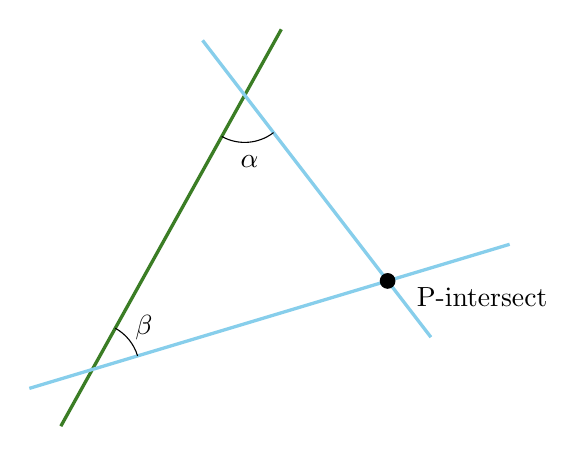
\begin{tikzpicture}
\draw[OliveGreen, very thick] (-0.4,-0.72) -- (2.4,4.32);
\draw[SkyBlue, very thick] (-0.8,-0.24) -- (5.3,1.59);
\draw[SkyBlue, very thick] (1.4,4.18) -- (4.3,0.41);
\coordinate (L) at (0,0);
\coordinate (T) at (1.935,3.484);
\coordinate (R) at (3.75,1.125);
\draw pic["$\beta$",draw,-,angle eccentricity=1.4, angle radius=0.6cm]{angle=R--L--T};
\draw pic["$\alpha$",draw,-,angle eccentricity=1.4, angle radius=0.6cm]{angle=L--T--R};
\fill[] (R) circle [radius=0.1];
\node[] at (3.75+1.2,1.125-0.2) {P-intersect};
\end{tikzpicture}
\end{center}
\end{enumerate}

\newpage

{\bf{}\Large DISCOVERY OF NON-EUCLIDEAN GEOMETRY}

\vspace{10pt}

Assuming that postulates 1 through 4 are true, the following are equivalent definitions of postulate 5;

\begin{enumerate}[label=(\alph*)]
\item Two parallels are equidistant.
\item If a line intersects one of two paralllels, then it intersects the other.
\item Given a triangle, a similar triangle can be constructed of any size.
\item The angular sum of a triangle is $180^\circ$.
\end{enumerate}

\vspace{10pt}

Saccheri's attempt to prove the parallel postulate let to many theorems - which he rejected for being repugnant to the nature of a straight line - which were actually true in hyperbolic geometry!


\begin{center}
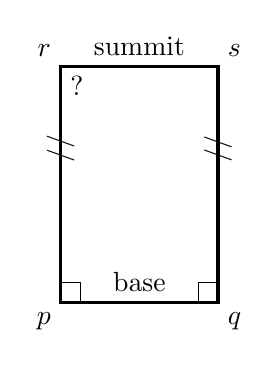
\begin{tikzpicture}[scale=2]
\draw[very thick] (0,0) -- node[pos=0.65,sloped]{//} (0,1.5) -- node[above,pos=0.5]{summit} (1,1.5) -- node[pos=0.35,sloped]{//} (1,0) -- node[above,pos=0.5]{base} (0,0) -- cycle;
\coordinate (P) at (0,0);
\coordinate (R) at (0,1.5);
\coordinate (S) at (1,1.5);
\coordinate (Q) at (1,0);
\draw pic["",draw,-,angle eccentricity=1.4, angle radius=0.25cm]{right angle=S--Q--P};
\draw pic["",draw,-,angle eccentricity=1.4, angle radius=0.25cm]{right angle=Q--P--R};
\node[below right] at (R) {?};
\node[below left] at (P) {$p$};
\node[above left] at (R) {$r$};
\node[above right] at (S) {$s$};
\node[below right] at (Q) {$q$};
\end{tikzpicture}
\end{center}

\vspace{10pt}

He was able to prove that $\angle r=\angle s$. Euclid's postulate is equivalent to $\angle r=90^\circ$, so Saccheri set about treating separately angles of $r$ which were obtuse and acute. Obtuse angles of $r$ led to a contradiction, but treatment of $r$ as though it were acute gave birth to the aforementioned theorems.

\vspace{10pt}

In hyperbolic geometry;

\begin{enumerate}[label=(\alph*)]
\item There are an {\bf{}infinite} number of parallel lines through a given point not on a line.
\item The lines mentioned in the parallel postulate do {\bf{}not} have to meet.
\item Two coplanar lines are {\bf{}never} equidistant.
\item A line may intersect one of two parallel lines, not {\bf{}not} necessarily the other.
\item Two similar triangles are always congruent.
\item The sum of the angles of a triangle is {\bf{}less} than $180^\circ$.
\end{enumerate}

\newpage

\underline{Further Developments}

\begin{enumerate}[label=$\rightarrow$]
\item projective geometry
\begin{itemize}\item no parallel lines\end{itemize}
\item Affine geometry
\begin{itemize}\item the geometry of  linear algebra\end{itemize}
\item multidimensional geometries
\item Differential geometry
\begin{itemize}\item geometry of curved surfaces (and lines)\end{itemize}
\end{enumerate}

\vspace{10pt}

There are no parallel lines in spherical (A.K.A elliptic) geometry, the angularsum of a trianlge exceeds $180^\circ$. As in hyperbolic geometry, similar triangles are congruent. Postulates 1. and 2. needed modification, as lines here are not infinite and two points can determine more than one line.

\chapter{COMPLEX NUMBERS}

A complex number is a point $z=(x,y)$ in the Cartesian plane in which the $x$-axis is measured in ordinary (real) units and the $y$-axis is measured in a different (imaginary) unit $i$, where $i^2=-1$. $x=\mbox{Re}(z)$, and $y=\mbox{Im}(z)$. NOTE that the real and imaginary components of $z$ are REAL numbers (they are coefficients).

\begin{center}
\begin{tikzpicture}[]
\begin{axis}[
standard,
xmin=0, xmax=4,
ymin=0, ymax=3,
xtick={0.5,1,1.5,2,2.5,3,3.5,4}, ytick={0.5,1,1.5,2,2.5,3},
xticklabels={,1,,2,,3,,4}, yticklabels={,$i$,,$2i$,,$3i$},
xlabel={$x$}, ylabel={$y$},
clip=false
]
\draw[dashed] (0,1.3) -- node[pos=0.5,above]{$x$} (2.3,1.3) -- node[pos=0.5,right]{$iy$} (2.3,0);
\fill[] (2.3,1.3) circle [x radius=0.08, y radius=0.06] node[right=3pt] {$z=(x,y)=x+iy$};
\fill[] (1,2.5) circle [x radius=0.08, y radius=0.06] node[right=3pt] {$(1,2.5)=1+2.5i$};
\end{axis}
\end{tikzpicture}
\end{center}

\newpage

{\bf{}\Large OPERATIONS ON COMPLEX NUMBERS}

\vspace{10pt}

Complex numbers inherit properties of vector addition (i.e. the parallelogram law) and scalar multiplication. Scalar multiplication of a complex number by a real number simply multiplies both components by the scalar coefficient.

\vspace{20pt}

\begin{tabular}{lll}
& {\bf{}Algebra} & {\bf{}Geometry}\\
$\begin{aligned}\multicolumn{1}{l}{\mbox{{\bf{}vector}}}\\\multicolumn{1}{l}{\mbox{{\bf{}addition:}}}\end{aligned}$ & $\begin{aligned}\multicolumn{1}{l}{$z=(x,y)\quad w=(s,t)$}\\\multicolumn{1}{l}{$z+w=(x+s,y+t)$}\end{aligned}$
&
\raisebox{-1cm}{
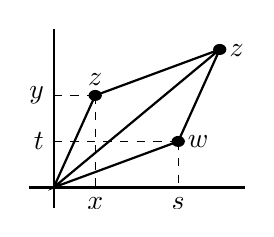
\begin{tikzpicture}[]
\begin{axis}[
scale=0.4,
standard,
xmin=0, xmax=4,
ymin=0, ymax=3,
xtick={\empty}, ytick={\empty},
axis line style={-}
]
\draw[thick] (0,0) -- (1,2) -- (4,3) -- (3,1) -- (0,0) -- (4,3);
\fill[] (1,2) circle [x radius=0.08*2, y radius=0.06*2] node[above]{$z$};
\fill[] (3,1) circle [x radius=0.08*2, y radius=0.06*2] node[right]{$w$};
\fill[] (4,3) circle [x radius=0.08*2, y radius=0.06*2] node[right]{$z+w$};
\draw[dashed] (0,1) -- (3,1) node[pos=0,left]{$t$};
\draw[dashed] (0,2) -- (1,2) node[pos=0,left]{$y$};
\draw[dashed] (1,2) -- (1,0) node[pos=1,below]{$x$};
\draw[dashed] (3,1) -- (3,0) node[pos=1,below]{$s$};
\end{axis}
\end{tikzpicture}}\\[5em]
$\begin{aligned}\multicolumn{1}{l}{\mbox{{\bf{}scalar}}}\\\multicolumn{1}{l}{\mbox{{\bf{}multiplication:}}}\end{aligned}$ & $\begin{aligned}\multicolumn{1}{l}{$z=(x,y)\quad (k\mbox{ real})$}\\\multicolumn{1}{l}{$kz=(kx,ky)$}\end{aligned}$
&
\raisebox{-1cm}{
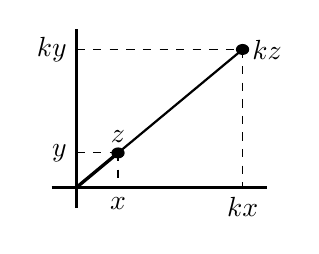
\begin{tikzpicture}[]
\begin{axis}[
scale=0.4,
standard,
xmin=0, xmax=4,
ymin=0, ymax=3,
xtick={\empty}, ytick={\empty},
axis line style={-},
clip=false
]
\draw[thick] (0,0) -- (4,3);
\draw[very thick] (0,0) -- (1,0.75) node[above]{$z$};
\fill[] (4,3) circle [x radius=0.08, y radius=0.06] node[right]{$kz$};
\fill[] (1,0.75) circle [x radius=0.08*2, y radius=0.06*2];
\fill[] (4,3) circle [x radius=0.08*2, y radius=0.06*2];
\draw[dashed] (0,0.75) -- (1,0.75) node[pos=0,left]{$y$};
\draw[dashed] (1,0.75) -- (1,0) node[pos=1,below]{$x$};
\draw[dashed] (0,3) -- (4,3) node[pos=0,left]{$ky$};
\draw[dashed] (4,3) -- (4,0) node[pos=1,below]{$kx$};
\end{axis}
\end{tikzpicture}}
\end{tabular}

\vspace{10pt}

Using  vector addition and scalar multiplication, we can write the complex number $z=(x,y)=x(1,0)+y(0,1)=x+iy$, where $z=x+iy$ is its Cartesian representation.

\vspace{10pt}

Questions:

\begin{enumerate}[label=\Alph*-]
\item find Cartesian form
\begin{enumerate}[label=(\alph*)]
\item $(2+3i)+(1-6i)=3-3i$
\item $4(-2+5i)-(-7-2i)=-1+22i$
\end{enumerate}
\item explain the commutative property of complex addition algebraically and geometrically
\begin{enumerate}[label=(\alph*)]
\item $\begin{aligned}[t](a+bi)+(c+di)&=(c+di)+(a+bi)\\(a+c)+(b+d)i&=(c+a)+(d+b)i\end{aligned}$

\vspace{10pt}

We have reduced complex addition to the addition of the real number components, treated as scalar coefficients. Therefore, by the commutative property of real numbers, complex addition too is commutative.
\item Per the parallelogram law, complex addition is commutative.
\end{enumerate}
\end{enumerate}

\newpage

{\bf{}\Large RELATED GEOMETRIC NOTIONS}

\vspace{10pt}

Worthy of special note is the modulus.

\vspace{20pt}

\begin{tabular}{lll}
& {\bf{}Algebra} & {\bf{}Geometry}\\[1em]
{\bf{}modulus:} & $|z|=\sqrt{x^2+y^2}$
&
\raisebox{-1cm}{
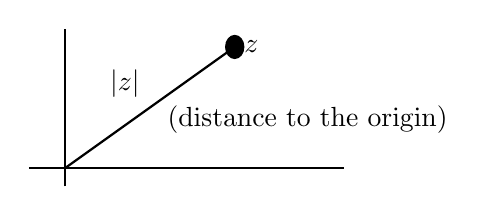
\begin{tikzpicture}[]
\begin{axis}[
width=5cm,
height=2.5cm,
scale only axis=true,
scale=0.8,
standard,
xmin=0, xmax=5,
ymin=0, ymax=2,
xtick={\empty}, ytick={\empty},
axis line style={-},
clip=false]
\draw[thick] (0,0) -- node[pos=0.5,above left]{$|z|$} (3.5,2);
\fill[] (3.5,2) circle [radius=0.2] node[right]{$z$};
\node[right=0.1cm] at (1.75,0.8) {(distance to the origin)};
\end{axis}
\end{tikzpicture}}\\[5em]
$\begin{aligned}\multicolumn{1}{l}{\mbox{{\bf{}distance}}}\\\multicolumn{1}{l}{\mbox{{\bf{}between}}}\\\multicolumn{1}{l}{\mbox{{\bf{}points:}}}\end{aligned}$ & $|z-w|=\sqrt{(x-s)^2+(y-t)^2}$
&
\raisebox{-1cm}{
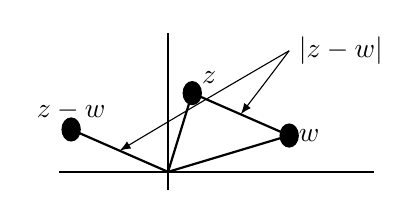
\begin{tikzpicture}[]
\begin{axis}[
width=5cm,
height=2.5cm,
scale only axis=true,
scale=0.8,
standard,
xmin=-1.5, xmax=3.5,
ymin=0, ymax=2,
xtick={\empty}, ytick={\empty},
axis line style={-},
clip=false]
\draw[thick] (0,0) -- (0.5,1.3);
\fill[] (0.5,1.3) circle [radius=0.2] node[above right]{$z$};
\draw[thick] (0,0) -- (2.5,0.6);
\fill[] (2.5,0.6) circle [radius=0.2] node[right]{$w$};
\draw[thick] (2.5,0.6) -- (0.5,1.3);
\draw[thick] (0,0) -- (-2,0.7);
\fill[] (-2,0.7) circle [radius=0.2] node[above]{$z-w$};
\node[right] at (2.5,2){$|z-w|$};
\draw[-latex] (2.5,2) to [bend right=1/3] (-1,0.35);
\draw[-latex] (2.5,2) to [bend left=1/3] (1.5,0.95);
\end{axis}
\end{tikzpicture}}\\[5em]
{\bf{}conjugate:} & $\bar{z}=x-iy$
&
\raisebox{-1cm}{
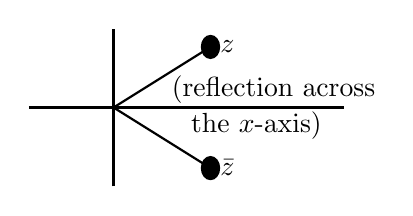
\begin{tikzpicture}[]
\begin{axis}[
width=5cm,
height=2.5cm,
scale only axis=true,
scale=0.8,
standard,
xmin=-1, xmax=4,
ymin=-1, ymax=1,
xtick={\empty}, ytick={\empty},
axis line style={-},
clip=false]
\draw[thick] (0,0) -- (2,1);
\fill[] (2,1) circle [radius=0.2] node[right]{$z$};
\draw[thick] (0,0) -- (2,-1);
\fill[] (2,-1) circle [radius=0.2] node[right]{$\bar{z}$};
\node[right] at (1,0.3) {(reflection across};
\node[right] at (1.4,-0.3) {the $x$-axis)};
\end{axis}
\end{tikzpicture}}
\end{tabular}

\vspace{10pt}

Themodulus has two important properties:

\begin{enumerate}[label=(\alph*)]
\item Homogeneity: $|kz|=|k||z|$ (where $k$ is real)
\item Triangular Inequality: $|z+w|\leq|z|+|w|$
\end{enumerate}

\vspace{10pt}

According to Euclidean geometry, one side of a triangle is always less than or equal to the sum of the other sides. This proves the triangle inequality.

\newpage

Questions:

\begin{enumerate}
\item[C-] Let $z=2+i$. Plot $z$, $-z$, $\bar{z}$, and $-\bar{z}$ on the same pair of axes. What shape is outlines? Note its relation to the coordinate axes.
\begin{center}
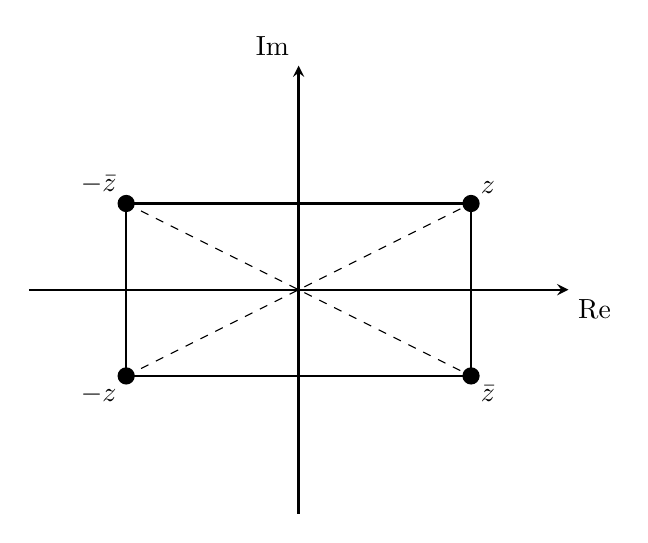
\begin{tikzpicture}
\begin{axis}[
axis equal,
standard,
xmin=-2, xmax=2,
ymin=-2, ymax=2,
xlabel={Re}, ylabel={Im},
xtick={\empty}, ytick={\empty},
]
\draw[thick] (2,1) -- (2,-1) -- (-2,-1) -- (-2,1) -- cycle;
\draw[dashed] (-2,-1) -- (2,1);
\draw[dashed] (-2,1) -- (2,-1);
\fill[] (2,1) circle [radius=0.1] node[above right]{$z$};
\fill[] (2,-1) circle [radius=0.1] node[below right]{$\bar{z}$};
\fill[] (-2,-1) circle [radius=0.1] node[below left]{$-z$};
\fill[] (-2,1) circle [radius=0.1] node[above left]{$-\bar{z}$};
\end{axis}
\end{tikzpicture}
\end{center}

The shape outlined by the positive and negative complex point-conjugate pairs is a rectangle that is centered at the origin. Due to this, it is symmetric about both coordinate axes.
\item[D-] What is $|2+i|$?

$z=2+i=2(1,0)+1(0,1)=(2,1)$, so $|z|=\sqrt{2^2+1^2}=\sqrt{5}$.
\end{enumerate}

\vspace{10pt}

{\bf{}\Large COMPLEX MULTIPLICATION}

\vspace{10pt}

Let $z=x+iy$ and $w=s+it$. Then, $zw=(x+iy)(s+it)=(xs-yt)+i(ys+xt)$.
Questions:

\begin{enumerate}
\item[E-] Evaluate products.
\begin{enumerate}[label=(\alph*)]
\item $i^2=-1$ by definition. More interesting is the polar transformation.
\item $(1+i)^2=1+2i+i^2=2i$
\item $(4+5i)(1-i)=4-4i+5i-5i^2=9+i$
\end{enumerate}
\end{enumerate}

\newpage

{\bf{}\Large POLAR FORM}

\vspace{10pt}

Every nonzero complex number has two square roots. This can be proven algebraically, but is also a simple consequence of geometric complex multiplication - which depends on understanding the polar form of complex numbers, as derived by Euler's formula.

\vspace{10pt}

We can use the modulus and basic trig definitions to re-express $z$ in a form which can be converted into a polar exponential using Euler's formula. The polar angle is in standard position.

\vspace{10pt}

\begin{tabular}{lll}
{\bf{}Polar form:} & $\begin{aligned}[b]z&=x+iy\\&=r\cos(\theta)+ir\sin(\theta)\\&=r(\cos(\theta)+i\sin(\theta))\\&=|z|e^{i\theta}\end{aligned}$
&
\raisebox{-0.4cm}{
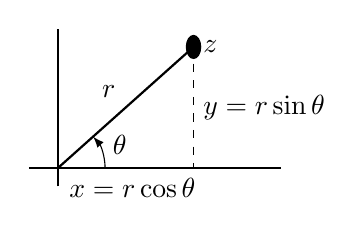
\begin{tikzpicture}[]
\begin{axis}[
width=4cm,
height=2.5cm,
scale only axis=true,
scale=0.8,
standard,
xmin=0, xmax=5,
ymin=0, ymax=2,
xtick={\empty}, ytick={\empty},
axis line style={-},
clip=false]
\coordinate (O) at (0,0);
\coordinate (Z) at (3.5,2);
\coordinate(X) at (Z |- O);
\draw[thick] (0,0) -- node[pos=0.5,above left]{$r$} (3.5,2);
\fill[] (3.5,2) circle [radius=0.2] node[right]{$z$};
\draw pic["$\theta$",draw,-latex,angle eccentricity=1.4, angle radius=0.6cm,trig format = deg]{angle=X--O--Z};
\draw[dashed] (Z) -- (X) node[pos=0.5,right]{$y=r\sin\theta$};
\path[] (O) -- (X) node[pos=0.55,below]{$x=r\cos\theta$};
\end{axis}
\end{tikzpicture}}
\end{tabular}

\vspace{10pt}

Euler's identity can be derived without the use of Taylor's Series by differentiating $f(\theta)=e^{-i\theta}(\cos\theta+i\sin\theta)$ to prove it is constant, finding that constant (1), and finally multiplying both sides of the equality by $e^{i\theta}$. Algebraically, it makes sense that multiplication by $i$ yields a 90 degree rotation of the point about the origin, because "the magnitude of the real and imaginary parts swap, and the real part of the new number is negative." I'll omit the trigonometricproof, as it is trivial.

\begin{center}
\begin{tikzpicture}
\begin{axis}[
standard,
xmin=-3, xmax=3,
ymin=0, ymax=3,
xtick={-3,2}, ytick={2,3},
xticklabels={$-b$,$a$}, yticklabels={$a$,$b$},
axis equal,
xlabel={Re}, ylabel={Im}
]
\coordinate (O) at (0,0);
\coordinate (P1) at (2,3);
\coordinate (P2) at (-3,2);
\draw[] (O) -- (P1) node[pos=0.5,above left]{$|z|$};
\draw[] (O) -- (P2) node[pos=0.5,above right]{$|z|$};
\draw pic["",draw,-,angle eccentricity=1.4, angle radius=0.4cm]{right angle=P1--O--P2};
\draw[dashed] (0,3) -- (P1) -- (2,0);
\draw[dashed] (-3,0) -- (P2) -- (0,2);
\end{axis}
\end{tikzpicture}
\end{center}

\newpage

\textit{Very} importantly, the fundamental properties of exponentiation hold for complex exponents.

\begin{align*}
e^ze^w&=e^{z+w}\\
e^{i\theta}e^{i\mu}&=(\cos\theta+i\sin\theta)(\cos\mu+i\sin\mu)\\
&=(\cos\theta\cos\mu-\sin\theta\sin\mu)+i(\sin\theta\cos\mu+\cos\theta\sin\mu)\\
&=\cos(\theta+\mu)+i\sin(\theta+\mu)\\
&=e^{i(\theta+\mu)}
\end{align*}

\vspace{10pt}

It is useful to define an operation which finds the angle of a complex number in standard position, this operation is called the {\bf{}argument} of $z$.

\[\arg(z)=\theta\quad\mbox{(mod 2$\pi$)}\]

\vspace{10pt}

Questions:

\begin{enumerate}
\item[F-] find the polar form
\begin{enumerate}[label=(\alph*)]
\item $1+i$

$\theta=\arctan(1)=\frac{\pi}{4}\mbox{ and }|z|=\sqrt{1^2+1^2}=\sqrt{2}\mbox{ so, }1+i=\sqrt{2}e^{\frac{\pi}{4}\cdot i}$
\item $1-i$

$\theta=\arctan(-1/1)=\arctan(-1)=-\frac{\pi}{4}\mbox{ and }|z|=\sqrt{1^2+(-1)^2}=\sqrt{2}\mbox{ so, }1-i=\sqrt{2}e^{-\frac{\pi}{4}\cdot i}$
\end{enumerate}
\end{enumerate}

\newpage

{\bf{}\Large THE GEOMETRY OF COMPLEX MULTIPLICATION}

\vspace{10pt}

Since multiplying complex numbers in their exponential form just multiplies their moduli and adds their angles, we can visualize the geometry of this quite easily. That is, if $z=|z|e^{i\theta}$and $w=|w|e^{i\mu}$, then $zw=|z||w|e^{i(\theta+\mu)}$.


\begin{center}
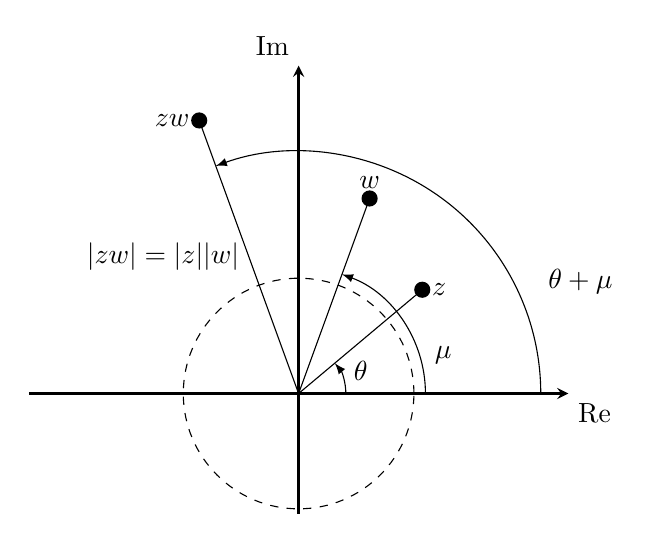
\begin{tikzpicture}
\begin{axis}[
standard,
xmin=-1.8, xmax=1.8,
ymin=0, ymax=1.8,
xtick={\empty}, ytick={\empty},
%xticklabels={$-1$,$1$}, yticklabels={$-1$,$1$},
axis equal,
xlabel={Re}, ylabel={Im},
trig format=deg,
clip = false
]
\draw[dashed] (0,0) circle [radius=1];
\coordinate (O) at (0,0);
\coordinate (P1) at (40:1.4);
\coordinate (P2) at (70:1.8);
\coordinate (P3) at (110:2.52);

\draw[] (0,0) -- (P1);
\fill[] (P1) circle [radius=0.07] node[right]{$z$};
\draw[] (0,0) -- (P2);
\fill[] (P2) circle [radius=0.07] node[above]{$w$};
\draw[] (0,0) -- (P3) node[pos=0.5,left]{$|zw|=|z||w|$};
\fill[] (P3) circle [radius=0.07] node[left]{$zw$};

\coordinate (X) at (1,0);

\draw pic["$\theta$",draw,-latex,angle eccentricity=1.4, angle radius=0.6cm]{angle=X--O--P1};
\draw[-latex] (1.1,0) arc [start angle=0, end angle=70, radius=1.1] node[pos=0.25, right=-0.6cm]{$\mu$};
\draw[-latex] (2.1,0) arc [start angle=0, end angle=110, radius=2.1] node[pos=0.25, right=-0.6cm]{$\theta+\mu$};
\end{axis}
\end{tikzpicture}
\end{center}

\vspace{10pt}

A basic formula that is still worth remembering is

\[\arg(zw)=\arg(z)+\arg(w)\quad\mbox{(mod 2$\pi$)}\]

\vspace{10pt}

{\bf{}Complex Arithmetic}

\begin{enumerate}[label=\arabic*)]
\item Find the Cartesian form of these complex numbers:
\begin{enumerate}[label=(\alph*)]
\item $4(1+2i)-2(5-i)=4+8i-10+2i=-6+10i$
\item $(1+i\sqrt{2})+\sqrt{2}(\pi+i)=1+\pi\sqrt{2}+i(\sqrt{2}+1)$
\item $2(4+i)-(1+6i)=7-4i$
\item $(1-2(i+3(1-4i)))=-5+22i$
\end{enumerate}
\item Find the Cartesian form of these complex numbers:
\begin{enumerate}[label=(\alph*)]
\item $(1+i)(1-i)=2$
\item $(5+10i)(-2+3i)=-40-5i$
\item $(1+i)^3=-2+2i$
\item $(1+2i)(3-4i)(5+6i)=(11+2i)(5+6i)=43+76i$
\end{enumerate}
\newpage
\item Prove these properties of the conjugate and the modulus:
\begin{enumerate}[label=(\alph*)]
\item $|kz|=|k||z|\ \mbox{($k$ real)}$

\begin{align*}
|kz|&=|k\mbox{Re}(z)+ik\mbox{Im}(z)|\\
&=\sqrt{(k\mbox{Re}(z))^2+(k\mbox{Im}(z))^2}\\
&=\sqrt{k^2(\mbox{Re}(z))^2+k^2(\mbox{Im}(z))^2}\\
&=\sqrt{k^2((\mbox{Re}(z))^2+(\mbox{Im}(z))^2))}\\
&=\sqrt{k^2}\sqrt{(\mbox{Re}(z))^2+(\mbox{Im}(z))^2)}\\
&=|k||z|
\end{align*}

And this is consistent with all of the geometric notions.

\begin{enumerate}[label=\roman*)]
\item This is the vector addition of parallel position vectors, $k$ times. This is equivalent to scalar multipication.
\item This is consistent with multiplying the components in scalar multiplication to recieve a "scaled" vector.
\item This is also consistent with polar multiplication, as we multiply the magnitudes, and add the angles, one of which is zero.
\end{enumerate}

\item $|z|^2=z\bar{z}$

\begin{align*}
|z|^2&=(\sqrt{(\mbox{Re}(z))^2+(\mbox{Im}(z))^2})^2\\
&=(\mbox{Re}(z))^2+(\mbox{Im}(z))^2\\
&=(\mbox{Re}(z))^2-(i\mbox{Im}(z))^2\\
&=(\mbox{Re}(z)+i\mbox{Im}(z))(\mbox{Re}(z)-i\mbox{Im}(z))\\
&=z\bar{z}
\end{align*}

This also makes geometric sense when multiplying in their polar forms, considering that the angles are additive inverses and the moduli being equal are squared.

\item $|wz|=|w||z|$

\begin{enumerate}

\item[proof 1:]

\[\mbox{Let }a=\mbox{Re}(w);\quad b=\mbox{Im}(w);\quad c=\mbox{Re}(z);\quad d=\mbox{Im}(z)\]

\begin{align*}
|wz|&=\sqrt{(ac-bd)^2+(ad+cb)^2}\\
&=\sqrt{a^2c^2-2acbd+b^2d^2+a^2d^2+adcb+c^2b^2}\\
&=\sqrt{a^2c^2+a^2d^2+b^2c^2+b^2d^2}\\
&=\sqrt{(a^2+b^2)(c^2+d^2)}\\
&=\sqrt{a^2+b^2}\sqrt{c^2+d^2}\\
&=|w||z|
\end{align*}

Geometrically, this can be explained in the light of polar form multiplication. In polar multiplication, we multiply the moduli and add the angles; this results in a complex number whos modulus is equal to the product of the moduli of its factors.

\item[proof 2:]

\[\mbox{Let }z=x+iy=|z|e^{i\theta};\quad w=u+iv=|w|e^{i\phi}\]

\begin{align*}
|zw|&=||z|e^{i\theta}|w|e^{i\phi}|=|z||w||e^{i\theta}||e^{i\phi}|\\
&=|z||w|\cdot1\cdot1=|z||w|
\end{align*}

\color{red}*only valid if 5(a) is proved\color{black}

\end{enumerate}

\item $\overline{zw}=\bar{z}\bar{w}$

\[\mbox{Let }a=\mbox{Re}(z);\quad b=\mbox{Im}(z);\quad c=\mbox{Re}(w);\quad d=\mbox{Im}(w)\]

\begin{align*}
\overline{zw}&=(ac-bd)-i(ad+cb)\\
&=ac+bdi^2-adi-cbi\\
&=(a-bi)(c-di)\\
&=\bar{z}\bar{w}
\end{align*}

This makes complete geometric sense. The product of two complex numbers is at an angle with is the sum of each of their arguments. The product of their conjugates has an angle which is the sum of their negated arguments. That is, they are symmetric about the Re axis. And since they are of equal magnitude, we can deduce that they are indeed conjugates of each other.
\end{enumerate}

\item Verify algebraically that complex multiplication satisfies the  distributive law: $z(w+u)=zw+zu$.

This is the product of a binomial and the sum of two other binomials.

\begin{align*}
z(w+u)&=(\mbox{Re}(z)+i\mbox{Im}(z))((\mbox{Re}(w)+i\mbox{Im}(w))+(\mbox{Re}(u)+i\mbox{Im}(u)))\\
&=(((\mbox{Re}(z)+i\mbox{Im}(z))(\mbox{Re}(w)+i\mbox{Im}(w)))+((\mbox{Re}(z)+i\mbox{Im}(z))(\mbox{Re}(u)+i\mbox{Im}(u))))\\
&=zw+zu
\end{align*}

And we could do it in polar form too by exponentiating to the arguments.
\end{enumerate}

\vspace{10pt}

{\bf{}Complex Arithmetic}

\begin{enumerate}
\item[5)] Evaluate these exponentials (that is, express them in Cartesian and/or polar form):
\begin{enumerate}[label=(\alph*)]
\item $e^{1+i\pi}=\boxed{e\cdot e^{i\pi}}=\boxed{-e}$
\item $\boxed{e^{1\pi/2}}=\boxed{i}$
\item $e^{e^{\ln\pi+i\pi/2}}=\boxed{e^{i\pi}}=\boxed{-1}$
\end{enumerate}
\item[6)] Verify that the law of exponents (i.e. $e^ze^w=e^{z+w}$) holds with base $e$ and arbitrary complex exponents.

My proposed solution supposes this by saying $e^z=e^xe^{iy}$; what is a more fundamental way of saying this?

\[\mbox{Let }z=x+iy=|z|e^{i\theta};\quad w=u+iv=|w|e^{i\mu}\]

\begin{align*}
e^ze^w&=e^xe^{iy}e^ue^{iv}\\
e^{i\theta}e^{i\mu}&=(\cos\theta+i\sin\theta)(\cos\mu+i\sin\mu)\\
&=(\cos\theta\cos\mu-\sin\theta\sin\mu)+i(\sin\theta\cos\mu+\cos\theta\sin\mu)\\
&=\cos(\theta+\mu)+i\sin(\theta+\mu)\\
&=e^{i(\theta+\mu)}
\end{align*}

\item[7)] Revisit when have learned series
\item[8)] cosine(0) plus isin(0) = 1. also, exp(0)=1.
\end{enumerate}

\vspace{10pt}

{\bf{}Polar Form}

\begin{enumerate}

\item[9)] convert to polar form

\begin{enumerate}[label=(\alph*)]
\item $-1=e^{i\pi}$
\item $i\sqrt{3}=\sqrt{3}e^{\frac{\pi}{2}i}$
\item $4i=4e^{\frac{\pi}{2}i}$
\item $5-5i\sqrt{3}=\sqrt{5^2+(5\sqrt{3})^2}e^{i\arctan(-5\sqrt{3}/5)}=10e^{i\arctan(-\sqrt{3})}=10e^{i\frac{\pi}{3}}$
\end{enumerate}

\item[10)] express in cartesian/polar form

\begin{enumerate}[label=(\alph*)]
\item $\frac{1}{i}=\frac{e^{0i}}{e^{\frac{\pi}{2}i}}=e^{0i-\frac{\pi}{4}i}=e^{-\frac{\pi}{2}i}$
\item $\frac{1}{1+i}=e^{0i}/e^{\frac{\pi}{4}i}=e^{-\frac{\pi}{4}i}$
\item $e^{\frac{\pi}{4}i}/e^{i\frac{\pi}{2}}=e^{-\frac{\pi}{4}i}$
\item 
\item
\end{enumerate}

\item[11)] use polar form to show that every complex number has a multiplicative inverse 1/z.

\[|z|e^{i\arg(z)}\cdot\frac{1}{|z|}e^{-i\arg(z)}=1\]

\item[12.] Use polar form to show that every complex number $z\neq0$ has two square roots.

\[\forall z=re^{i\theta}\in\mathbb{C}:z\neq0\exists w_1=\sqrt{r}e^{i\frac{\theta}{2}};\ w_2=\sqrt{r}e^{i\frac{\theta}{2}+\pi}:w_1^2=w_2^2=z\]

\end{enumerate}











\end{document}